%************************************************
\chapter{Introduction}\label{ch:introduction}
%************************************************
\section{Motivation}
In recent years, there has been a rise in the use of neuroimaging in the clinical practice. It has improved and speeded the procedure of diagnostic, providing unprecedented insight into the brain. Neuroimaging is very extended in research as well. Different fields such as psychiatry, neurology, psychology, behavioural science or biology make extensive use of brain imaging in their studies. 

The basis of these studies are common: a selection procedure by which a representative set of subjects is recruited, the fulfilment of an experiment on (or by) each subject and a statistical analysis of the acquired data. Particularly, when studying a certain disease, it is common to recruit subjects affected by the disease and non-affected, healthy subjects, usually known as \acp{CTL}. Then, in this typical example, both affected and \acp{CTL} are scanned, and brain anatomy or function is analysed using statistical tools. The result of this analysis is a list of significant differences between structure or function that could be linked to the disease. 

\ac{CAD} systems provide a set of tools to help setting up and performing these studies. It is currently a thriving area of research involving multidisciplinary teams, combining computer science, mathematics, medicine, artificial intelligence, statistics, machine learning, and many others \cite{Martinez-Murcia2016}. The main aim is to assist clinicians in the procedure of diagnosis and study of the diseases by providing software that can effectively recognize disease patterns, characterize differences and make predictions. 

One fundamental issue often found in this studies is the sample size. The number of subjects frequently ranges from tens to hundreds, whereas the number of features (namely voxels) to be analysed can add up to millions. This causes the so-called \emph{Small Sample Size Problem} \cite{Duin2000} which negatively affects the statistical power of any experiment performed using these datasets \cite{Button2013}. 

\begin{figure}
\centering
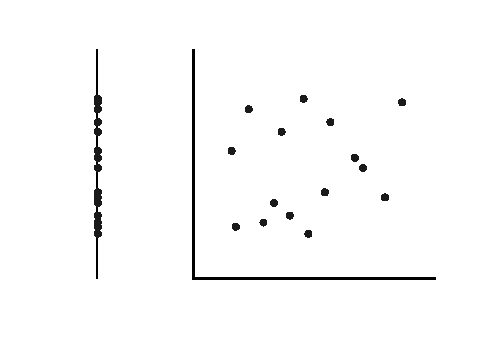
\includegraphics[width=0.6\linewidth]{Graphics/ch1/smallsample}
\caption[Illustration of one and two-dimensional spaces.]{Illustration of the separation between points in one-dimensional and two-dimensional spaces.}
\label{fig:smallsample}
\end{figure}


\section{The Small Sample Size Problem}\label{sec:smallsamplesize}
The \textit{Small Sample Size Problem} refers to a problem that arises when the proportion between number of subjects and number of features is large. Think of, \eg, 15 points in a one-dimensional line, as in Figure~\ref{fig:smallsample}. If we think of a subject as a vector, we would have 15 subjects in a one-dimensional space. Now, imagine that we add a second dimension. It is easy to see that our subjects would be farther than in the two-dimensional world. And the same would happen if we move to four, ten or thousands of dimensions. The farther our points are, the more difficult is for a statistical tool to extract information. That is what we call \textit{almost empty spaces} \cite{Stoeckel04}, in contrast to \textit{dense spaces}, where points are closer. 

Neuroimaging provides hundreds of thousands, or even millions of voxels, in what could mean millions of features. That implies that any calculation performed in those almost empty spaces will eventually lack information. This implies a loss of statistical power of the methods used, usually producing false negatives (the system is unable to detect real signal) and false positives (the system detects signal where there is not). These are known in statistics as Type I and Type II errors respectively. 

In differential diagnosis studies, the small sample size problem leads to wrong conclusions about where real differences are located. This, in addition to untracked confounding variables are one of the fundamental sources of non-re\-pro\-du\-ci\-bi\-li\-ty un current neuroimaging studies \cite{Button2013}. 

The solution might seem straightforward: increase sample size. But this is not always possible, since neuroimaging studies do their best at recruiting as many people as they can with a limited budget. Many efforts have been put into establishing multi-centre collaborations that allow the recruitment of a larger population, but despite offering a higher statistical power, these studies still suffer from a number of confounding variables such as population bias or scanner differences \cite{haar2014anatomical}. In Chapters~\ref{ch:swpca} and \ref{ch:simulation} we explore different approaches to this solution. 

Another option involves reducing the number of features, via feature selection or feature extraction. This has been widely used in computed-aided methodology for neuroimaging \cite{DeMartino2007,xu2009source,Gorriz2010,Illan2011,Martinez-Murcia2016} with great success, and solutions using this approach will be treated in Chapters~\ref{ch:decomposition}, \ref{ch:texture} and \ref{ch:sbm}. 

The Small Sample Size problem is directly related to the \textit{Curse of Dimensionality} \cite{Krishnaiah1982}, which proves that, in contrast to what could be expected, once a certain classifier performance has been achieved, it holds or even decreases when feeding more features to the classifier. The problem also affects statistical hypothesis testing, a tool widely used for inference in neuroimaging, in what is known as the \textit{Multiple Comparisons} problem \cite{Benjamini2010}, a particular field that is still being studied. 

% DONE
\section{Aims and Objectives}\label{sec:overview}
This thesis aims to contribute new approaches to overcome the small sample size problem in neuroimaging. This can provide more accurate \ac{CAD} systems by reducing the number of false positives, increasing the reliability of their results. 

We will take two different approaches, as commented in previous sections: increasing the sample size and reducing the feature space. Therefore, we can define the following objectives: 

\begin{itemize}
	\item Develop and evaluate algorithms that reduce the feature space, in which is usually known in the field as feature extraction and feature selection strategies. 
	\item Develop and evaluate new strategies to increase the sample size in neuroimaging studies. 
\end{itemize}

Many strategies have been proposed . 

In this thesis we plan to tackle the Small Sample Size problem in two different approaches. 


First strategy: decrease the number of features -> Feature extraction. This is the subject of Decomposition techniques, Texture Analysis and \ac{SBM}. 

Second strategy: increase the sample size. Most popular option: multi-site studies where subjects are acquired using similar techniques at different sites. This poses a major problem: inhomogeneities, etc. To overcome this we propose the \ac{SWPCA}. Other option: simulate new subjects from the existent database, in order to increase sample size.



The aim of the work, i.e. the overall purpose of the study, should be clearly and concisely defined.

Aims:
Are broad statements of desired outcomes, or the general intentions of the research, which 'paint a picture' of your research project
Emphasize what is to be accomplished (not how it is to be accomplished)
Address the long-term project outcomes, i.e. they should reflect the aspirations and expectations of the research topic.
Once aims have been established, the next task is to formulate the objectives. Generally, a project should have no more than two or three aims statements, while it may include a number of objectives consistent with them.

Objectives are subsidiary to aims and:

Are the steps you are going to take to answer your research questions or a specific list of tasks needed to accomplish the goals of the project
Emphasize how aims are to be accomplished
Must be highly focused and feasible
Address the more immediate project outcomes
Make accurate use of concepts
Must be sensible and precisely described
Should read as an 'individual' statement to convey your intentions
Here is an example of a project aim and subsidiary objectives:


Obj: provide more accurate CAD systems by reducing the number of false positives, increasing the reliability of their results. 

1 - Develop and evaluate different strategies for reducing the feature space. 
2 - Develop and evaluate different strategies for safely increasing the sample size. 

The overall goal of this thesis was to contribute to the emerging field of statistical eco-
toxicology, environmental risk assessment and environmental monitoring. The main
objectives were (i) to scrutinise new methods in statistical ecotoxicology and effect as-
sessment, (ii) explore risk dynamics using available monitoring data and (iii) provide
tools to deal with and integrate big data in ERA. Figure 1.1 provides a conceptual
overview on ERA and environmental monitoring as outlined in the previous sections,
as well as the parts considered in this thesis and their relationships.

\section{Contributions}
Some ideas and figures have appeared previously in the following publications, that we divide here in articles and conference presentations. 

%\noindent Put your publications from the thesis here. The packages \texttt{multibib} or \texttt{bibtopic} etc. can be used to handle multiple different bibliographies in your document.

\begin{refsection}[ownpubs]
	\small
	\nocite{*} % is local to to the enclosing refsection
	\newrefcontext[sorting=ydnt]
	\subsection{Articles}
	\printbibliography[env=nolabelbib,heading=none,keyword=own, title={Articles}, type=article]
	\subsection{Conferences}
	\printbibliography[env=nolabelbib,heading=none,keyword=own, title={Conferences}, type=inproceedings]
	\subsection{Books}
	\printbibliography[env=nolabelbib,heading=none,keyword=own, title={Books}, type=inbook]
\end{refsection}

\section{Organization of this Thesis}

\begin{figure}
\centering
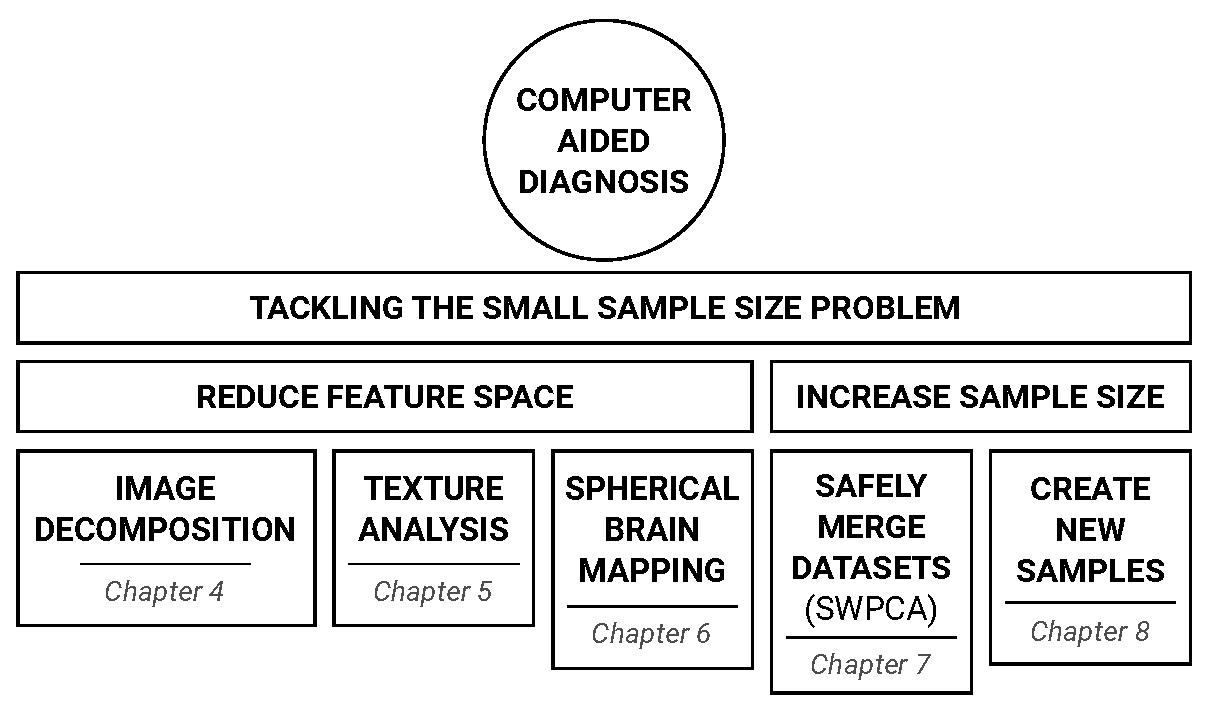
\includegraphics[width=0.7\linewidth]{Graphics/ch1/outline}
\caption[Structure of the thesis.]{Structure and connexions between the different strategies proposed in this thesis, organized by chapters and parts.}
\label{fig:outline}
\end{figure}

This thesis work is organized in four parts plus appendices, each of which is subdivided in several chapters. In the first part, we introduce the motivations and main aims of this work (Chapter~\ref{ch:introduction}), examine the state of the art in medicine, neuroimaging and \ac{CAD} systems (Chapter~\ref{ch:stateofart}) and present a general methodology that will be followed throughout this thesis, including preprocessing and evaluation (Chapter~\ref{ch:preprocessing}). 

Parts \ref{part:feature} and \ref{part:increase} refers to each of the solutions outlined above, and disaggregated in Figure~\ref{fig:outline}. In part~\ref{part:feature} we focus on the feature reduction techniques, including decomposition methods (Chapter~\ref{ch:decomposition}), texture analysis (Chapter~\ref{ch:texture}), and the novel algorithm Spherical Brain Mapping (Chapter~\ref{ch:sbm}). On the other hand, Part~\ref{part:increase} is focused on two different strategies used to increase the sample size: the Significance Weighted Principal Component Analysis algorithm (Chapter~\ref{ch:swpca}), used to safely merge structural images acquired at different centres, and a neuroimage simulation algorithm (Chapter~\ref{ch:simulation}) that can be used to extend existing functional datasets. 

Finally, in Part~\ref{part:dicussion} we provide a general discussion of the results presented in this thesis, conclusions about the methods and prospective work that could be performed with this basis. 
